%-----------------------------------------------%
%             filename: skeleton.tex
%-----------------------------------------------%
\documentclass[aps,twocolumn]{revtex4-1}
\usepackage{graphicx}
\usepackage{ifpdf}
\ifpdf
	\usepackage[backref]{hyperref}
	%\usepackage[backref,pageanchor=true,plainpages=false, pdfpagelabels,bookmarks,bookmarksnumbered]	{hyperref}
\else
\fi

\usepackage{crs}

% see http://goo.gl/5Fo27
\newtoggle{thmsty}
%\toggletrue{thmsty}
\togglefalse{thmsty}

% see http://goo.gl/7jLZ9
\makeatletter
\newlength \figwidth
\if@twocolumn
  \setlength \figwidth {0.8\columnwidth}
\else
  \setlength \figwidth {0.5\textwidth}
\fi
\makeatother

\begin{document} 

\title{\bf Abstract semantics for network representations of biological systems}

\author{a1$^{1}$, a2$^{1}$, a3$^{1}$, a4$^{1,2,3}$}

\affiliation{$^1$Department of Systems and Computational Biology,\\ $^2$Dominick P. Purpura Department of Neuroscience, \\ $^3$Department of Pathology, Albert Einstein College of Medicine, 1301 Morris Park Ave, Bronx, NY 10461, USA}

\date{\today}
\begin{abstract}
It has become standard to represent information collected about biological systems using "networks" or algebraic graphs. However, the semantics of such representations is often unclear with respect to biological function. As a result, it is difficult to understand such representations and therefore to construct a framework that would support the computation of various implications of information about biological systems represented in this format. Although efforts have been made to standardize such representations, they sometimes incorporate specific details that prevent the employment of potentially useful abstractions. Here we suggest an informal abstract semantics for representations of biological networks that we believe could support (automated) reasoning about biological systems from the perspective of their network representations. 
\end{abstract}

\maketitle

\tableofcontents

\section{Introduction}

\subsection{Network representations of biological systems}

\begin{figure*}
\noindent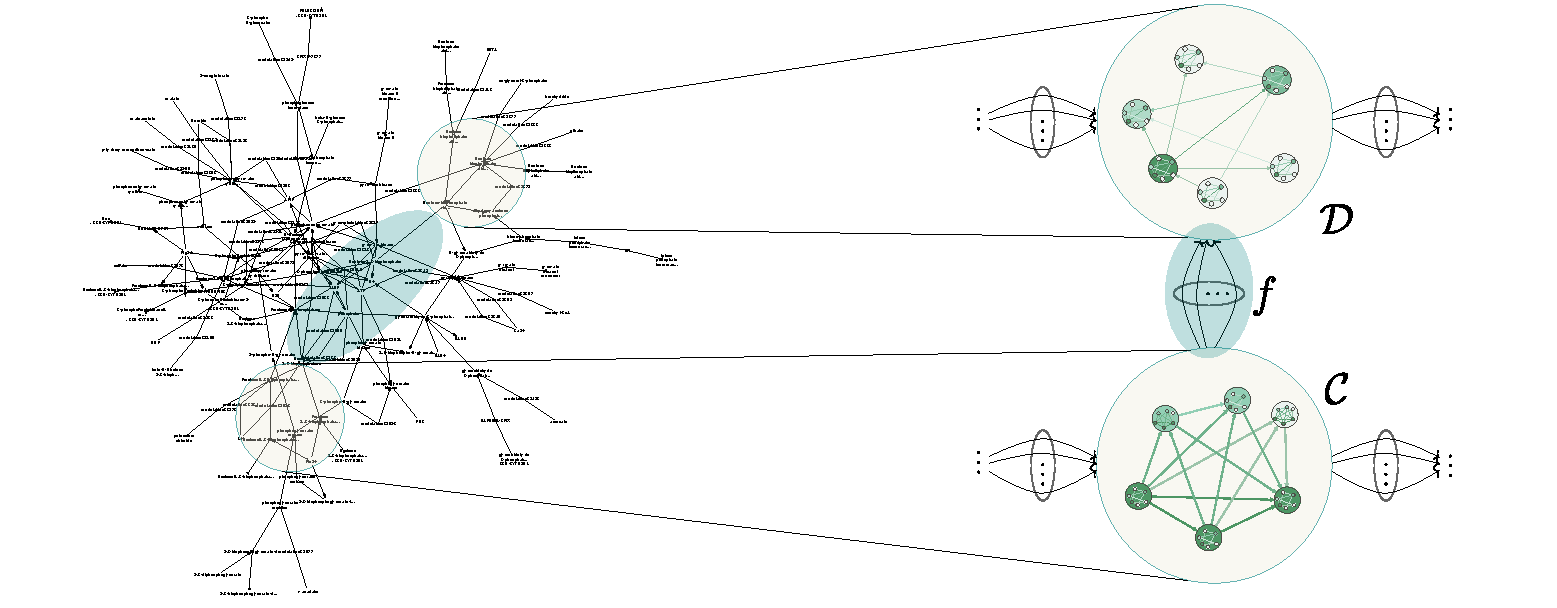
\includegraphics[width=1.9\columnwidth]{fig/biograph.pdf}
\caption{Particular features of interaction networks underlying biological systems can be abstracted as graphs of some type with morphisms translating structure between them.}
\label{fig:biograph}
\end{figure*}

At least since the advent of network science and perhaps before it has become common to represent various aspects of ostensible knowledge about biological systems such as protein-protein, DNA-protein, RNA-protein, RNA-RNA, inter-individual, inter-population, inter-community and other interactions using algebraic graphs of some flavor (e.g. undirected, directed, multi-, hyper-, and cell complexes among others). There has been an effort in the molecular context to standardize such representations using, for example, the so-called systems biology graphical notation among others \cite{LeNovere2009,Demir2010,Ghosh2011}. While these efforts may be helpful in some contexts, they have yet to be considered in a manner that balances biological knowledge with mathematical and computational knowledge regarding structures that can encapsulate data and support the computation of various pieces of information that can be derived from it. The purpose behind supporting the latter approach would be to render the representation that emerges susceptible to all of the analytical techniques that have been developed for reasoning about whatever particular type of structure may be chosen. Of course, ultimately the project of representing knowledge about biological systems may require the development of structures that have not been thought of yet in a mathematical or computational setting; however, taking as a point of departure \emph{ad hoc} structures upon which no framework for reasoning whatever has been developed would seem to be an inefficient approach given that there are in existence many such structures supporting very useful reasoning methods.

Given that biological systems may be concretely represented as graphs or a generalization thereof, we find that concepts from category theory may serve as a more flexible as well as mathematically and computationally well-supported point of departure for representing the kind of knowledge about biological systems that has come to be commonly expressed in terms of networks. We will recount more precise definitions in what follows, but we note here that all the letters representing categories and objects and morphisms between objects or categories can be specialized to categories where objects represent graphs, hypergraphs, and even more complicated structures that could be useful in representing information about biological networks. What is perhaps most important about this approach is that, upon subsequent specialization within a category theoretic representation to that of graphs or hypergraphs for example, the introduction of categories will have enabled support for precise reasoning about biological systems in terms of something that formalizes their colloquial network representations.


%------bibliography---%
\bibliographystyle{unsrt} 
\bibliography{bib/books,bib/papers}
%---------------------%


%-----------------------------------------------%
%                   appendix
%-----------------------------------------------%
\appendix
\section{Category theory}\label{app:CatTh}
\iftoggle{thmsty}{
\begin{definition}
\label{definition-category}
}{}
A {\it category} $\mathcal{C}$ is:
\begin{enumerate}
\item A set of objects $\Ob(\mathcal{C})$.
\item For each pair $x, y \in \Ob(\mathcal{C})$ a set of morphisms
$\Mor_\mathcal{C}(x, y)$.
\item For each triple $x, y, z\in \Ob(\mathcal{C})$ a composition
map $ \Mor_\mathcal{C}(y, z) \times \Mor_\mathcal{C}(x, y)
\to \Mor_\mathcal{C}(x, z) $, denoted $(\phi, \psi) \mapsto
\phi \circ \psi$.
\end{enumerate}
Such that these constraints are satisfied:
\begin{enumerate}
\item For every element $x\in \Ob(\mathcal{C})$ there exists a
morphism $\text{id}_x\in \Mor_\mathcal{C}(x, x)$ such that
$\text{id}_x \circ \phi = \phi$ and $\psi \circ \text{id}_x = \psi $.
\item Composition is associative, i.e., $(\phi \circ \psi) \circ \chi =
\phi \circ ( \psi \circ \chi)$.
\end{enumerate}
\iftoggle{thmsty}{
\end{definition}
}

\iftoggle{thmsty}{
\begin{definition}
\label{definition-functor}
}{}
A {\it functor} $F : \mathcal{A} \to \mathcal{B}$
between two categories $\mathcal{A}, \mathcal{B}$ is:
\begin{enumerate}
\item A map $F : \Ob(\mathcal{A}) \to \Ob(\mathcal{B})$.
\item For every $x, y \in \Ob(\mathcal{A})$ a map
$F : \Mor_\mathcal{A}(x, y) \to \Mor_\mathcal{B}(F(x), F(y))$,
denoted $\phi \mapsto F(\phi)$.
\end{enumerate}
These data should be compatible with composition and identity morphisms
in the following manner: $F(\phi \circ \psi) =
F(\phi) \circ F(\psi)$ for a composable pair $(\phi, \psi)$ of
morphisms of $\mathcal{A}$ and $F(\text{id}_x) = \text{id}_{F(x)}$.
\iftoggle{thmsty}{
\end{definition}
}

\iftoggle{thmsty}{
\begin{definition}
\label{definition-transformation-functors}
}{}
Let $F, G : \mathcal{A} \to \mathcal{B}$ be functors.
A {\it natural transformation}, or a {\it morphism of functors}
$t : F \to G$, is a collection $\{t_x\}_{x\in \Ob(\mathcal{A})}$
such that
\begin{enumerate}
\item $t_x : F(x) \to G(x)$ is a morphism in the category $\mathcal{B}$, and
\item for every morphism $\phi : x \to y$ of $\mathcal{A}$ the following
diagram is commutative
$$
\xymatrix{
F(x) \ar[r]^{t_x} \ar[d]_{F(\phi)} & G(x) \ar[d]^{G(\phi)} \\
F(y) \ar[r]^{t_y} & G(y) }
$$
\end{enumerate}
\iftoggle{thmsty}{
\end{definition}
}

We can define a category having functors as objects and natural transformations as morphisms, which is called a functor category, by recognizing that every functor $F$ comes with the {\it identity} transformation $\text{id}_F : F \to F$. In addition, given a morphism of
functors $t : F \to G$ and a morphism of functors $s : E \to F$
then the {\it composition} $t \circ s$ is defined by the rule
$$
(t \circ s)_x = t_x \circ s_x : E(x) \to G(x)
$$
for $x \in \Ob(\mathcal{A})$.
This is a morphism of functors
from $E$ to $G$.
Thus, given categories
$\mathcal{A}$ and $\mathcal{B}$ we obtain the category of functors between $\mathcal{A}$ and
$\mathcal{B}$.

\iftoggle{thmsty}{
\begin{definition}
\label{definition-equivalence-categories}
}{}
An {\it equivalence of categories}
$F : \mathcal{A} \to \mathcal{B}$ is a functor such that there
exists a functor $G : \mathcal{B} \to \mathcal{A}$ such that
the compositions $F \circ G$ and $G \circ F$ are isomorphic to the
identity functors $\text{id}_\mathcal{B}$,
respectively $\text{id}_\mathcal{A}$.
In this case we say that $G$ is a {\it quasi-inverse} to $F$.
\iftoggle{thmsty}{
\end{definition}
}

\iftoggle{thmsty}{
\begin{definition}
\label{definition-adjoint}
}{}
Let $\mathcal{C}$, $\mathcal{D}$ be categories.
Let $u : \mathcal{C} \to \mathcal{D}$ and
$v : \mathcal{D} \to \mathcal{C}$ be functors.
We say that $u$ is a {\it left adjoint} of $v$ or that
$v$ is a {\it right adjoint} to $u$, written $u \dashv v$, if there are bijections
$$
\phi_{X,Y}:\Mor_\mathcal{D}(u(X), Y)
\simeq
\Mor_\mathcal{C}(X, v(Y))
$$
functorial in $X \in \Ob(\mathcal{C})$, and
$Y \in \Ob(\mathcal{D})$.
\iftoggle{thmsty}{
\end{definition}
}

Morphisms that are associated with each other according to the bijections of an adjunction are called {\it adjoint transposes} of one another. If $g:u(X) \rightarrow Y$, $g \in \Mor(\cD)$ then $g^*: X \rightarrow v(Y)$, $g^* \in \Mor(\cC)$ is given by $\phi_{X,Y}(g) = g^*$. Similarly for $f: X \rightarrow v(Y)$, $f \in \Mor(\cC)$ with $f^*:u(X) \rightarrow Y$, $f^* \in \Mor(\cD)$ is given by $\phi_{X,Y}^{-1}(f) = f^*$. We see then that $g^* = f$ and $f^* = g$.

\iftoggle{thmsty}{
\begin{definition}
\label{definition-opposite}
}{}
Given a category $\mathcal{C}$ the {\it opposite category}
$\mathcal{C}^{opp}$ is the category with the same objects
as $\mathcal{C}$ but all morphisms reversed.
\iftoggle{thmsty}{
\end{definition}
}

\iftoggle{thmsty}{
\begin{definition}
\label{definition-contravariant}
}{}
Let $\mathcal{C}$, $\mathcal{S}$ be categories.
A {\it contravariant} functor $F$
from $\mathcal{C}$ to $\mathcal{S}$
is a functor $\mathcal{C}^{opp}\to \mathcal{S}$.
\iftoggle{thmsty}{
\end{definition}
}

\iftoggle{thmsty}{
\begin{definition}
\label{definition-presheaf}
}{}
Let $\mathcal{C}$ be a category.
\begin{enumerate}
\item A {\it presheaf of sets on $\mathcal{C}$}
or simply a {\it presheaf} is a contravariant functor
$F$ from $\mathcal{C}$ to $\textit{Sets}$. When $F$ is a covariant functor $F : \mathcal{C}^{opp} \rightarrow \textit{Sets}$.
\item The category of presheaves is denoted $\textit{PSh}(\mathcal{C})$.
\end{enumerate}
\iftoggle{thmsty}{
\end{definition}
}

\iftoggle{thmsty}{
\begin{definition}
\label{definition-products}
}{}

Let $x, y\in \Ob(\mathcal{C})$,
A {\it product} of $x$ and $y$ is
an object $x \times y \in \Ob(\mathcal{C})$
together with morphisms
$p\in \Mor_{\mathcal C}(x \times y, x)$ and
$q\in\Mor_{\mathcal C}(x \times y, y)$ such
that the following universal property holds: for
any $w\in \Ob(\mathcal{C})$ and morphisms
$\alpha \in \Mor_{\mathcal C}(w, x)$ and
$\beta \in \Mor_\mathcal{C}(w, y)$
there is a unique
$\gamma\in \Mor_{\mathcal C}(w, x \times y)$ making
the diagram
$$
\xymatrix{
w \ar[rrrd]^\beta \ar@{-->}[rrd]_\gamma \ar[rrdd]_\alpha & & \\
& & x \times y \ar[d]_p \ar[r]_q & z \\
& & x &
}
$$
commute.
\iftoggle{thmsty}{
\end{definition}
}

\iftoggle{thmsty}{
\begin{definition}
\label{definition-has-products-of-pairs}
}{}
We say the category $\mathcal{C}$ {\it has products of pairs
of objects} if a product $x \times y$
exists for any $x, y \in \Ob(\mathcal{C})$.
\iftoggle{thmsty}{
\end{definition}
}

\iftoggle{thmsty}{
\begin{definition}
\label{definition-coproducts}
}{}
Let $x, y \in \Ob(\mathcal{C})$,
A {\it coproduct}, or {\it amalgamated sum} of $x$ and $y$ is
an object $x \amalg y \in \Ob(\mathcal{C})$
together with morphisms
$i \in \Mor_{\mathcal C}(x, x \amalg y)$ and
$j \in \Mor_{\mathcal C}(y, x \amalg y)$ such
that the following universal property holds: for
any $w \in \Ob(\mathcal{C})$ and morphisms
$\alpha \in \Mor_{\mathcal C}(x, w)$ and
$\beta \in \Mor_\mathcal{C}(y, w)$
there is a unique
$\gamma \in \Mor_{\mathcal C}(x \amalg y, w)$ making
the diagram
$$
\xymatrix{
& y \ar[d]^j \ar[rrdd]^\beta \\
x \ar[r]^i \ar[rrrd]_\alpha & x \amalg y \ar@{-->}[rrd]^\gamma \\
& & & w
}
$$
commute.
\iftoggle{thmsty}{
\end{definition}
}

\iftoggle{thmsty}{
\begin{definition}
\label{definition-has-coproducts-of-pairs}
}{}
We say the category $\mathcal{C}$ {\it has coproducts of pairs
of objects} if a coproduct $x \amalg y$
exists for any $x, y \in \Ob(\mathcal{C})$.
\iftoggle{thmsty}{
\end{definition}
}

\iftoggle{thmsty}{
\begin{definition}
\label{definition-product-category}
}{}
Let $\mathcal{A}$, $\mathcal{B}$ be categories.
The {\it product category} is the category
$\mathcal{A} \times \mathcal{B}$ with
objects
$\Ob(\mathcal{A} \times \mathcal{B}) =
\Ob(\mathcal{A}) \times \Ob(\mathcal{B})$
and
$$
\Mor_{\mathcal{A} \times \mathcal{B}}((x, y), (x', y'))
:=
\Mor_\mathcal{A}(x, x')\times
\Mor_\mathcal{B}(y, y').
$$
Composition of morphisms is defined according to components.
\iftoggle{thmsty}{
\end{definition}
}

\iftoggle{thmsty}{
\begin{definition}
\label{definition-bifunctor}
}{}
Given categories $\mathcal{C}_1$, $\mathcal{C}_2$, and $\mathcal{D}$. A {\it bifunctor} or binary functor or 2-ary functor or functor of two variables, $F$, is a functor whose domain is the product of two categories $F: \mathcal{C}_1 \times \mathcal{C}_2 \rightarrow \mathcal{D}$.
\iftoggle{thmsty}{
\end{definition}
}

\iftoggle{thmsty}{
\begin{definition}
\label{definition-hom-functor}
}{}
The {\it hom-functor} is a bifunctor defined on the product of a category $\mathcal{C}$ with its self-dual category $\mathcal{C}^{opp}$, which takes values in the category $\textit{Sets}$. Thus for a category $C$ its hom-functor is 
$$
hom(-,-): \mathcal{C}^{opp} \times \mathcal{C} \rightarrow \textit{Sets},
$$
which can be curried in two ways
\begin{eqnarray*}
hom^{(-)} &:& \mathcal{C}^{opp} \rightarrow \textit{Sets}^{\mathcal{C}},\\
hom_{(-)} &:& \mathcal{C} \rightarrow \textit{Sets}^{\mathcal{C}^{opp}}.
\end{eqnarray*}
The hom-functor maps
\begin{enumerate}
\item objects $(c,c') \in \mathcal{C}^{opp} \times \mathcal{C}$ to the hom-set $\Mor_{\mathcal{C}} (c,c')$, which is the set of morphisms in $\mathcal{C}$ with domain $c$ and codomain $c'$.
\item morphisms 
$$
(f,g):(c,c') \rightarrow (d,d') \in \Mor(\mathcal{C}^{opp} \times \mathcal{C}),
$$
where $f:d \rightarrow c \in \Mor(\mathcal{C})$ and $g:c' \rightarrow d' \in \Mor(\mathcal{C})$, to the set function
\begin{eqnarray*}
\Mor_{\mathcal{C}}(c,c') &\rightarrow& \Mor_{\mathcal{C}}(d,d')\\
(c \rightarrow c') &\mapsto& (d \rightarrow c \rightarrow c' \rightarrow d')
\end{eqnarray*}
\end{enumerate}
\iftoggle{thmsty}{
\end{definition}
}

\iftoggle{thmsty}{
\begin{definition}
\label{definition-representable-functor}
}{}
For a hom-functor $hom(-,-): \mathcal{C}^{opp} \times \mathcal{C} \rightarrow \textit{Sets}$ for $c \in \Ob(\mathcal{C})$ a covariant and contravariant functor can be derived by specializing the hom-functor to morphisms out of or into the object $c$ as
\begin{eqnarray*}
h^c \equiv hom(-,c) &:& \mathcal{C}^{opp} \rightarrow \textit{Sets}\\
h_c \equiv hom(c,-) &:& \mathcal{C} \rightarrow \textit{Sets}.
\end{eqnarray*}
Functors that are isomorphic to $h^c$ or $h_c$ are referred to as {\it corepresentable or representable functors} respectively and $c$ is their {\it representing object}. Note that $h^c \in \Ob(\textit{PSh}(\mathcal{C}))$.
\iftoggle{thmsty}{
\end{definition}
}{}

\begin{figure}
\noindent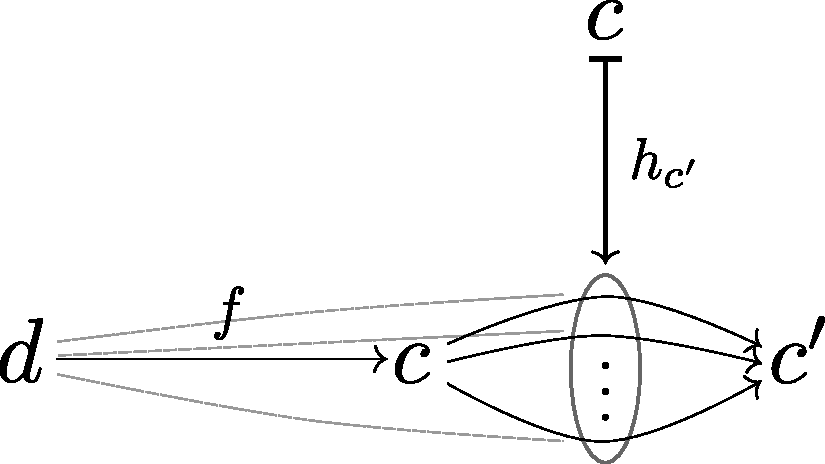
\includegraphics[width=0.7\columnwidth]{fig/hom.pdf}
\caption{The presheaf represented by $c' \in \Ob(\cC)$ is $h^{c'} : \cC^{opp} \rightarrow \textit{Sets}$. It sends objects to the set of morphisms in which they are the domain object with codomain $c'$ and morphisms $f:d \rightarrow c \in \Mor{\cC}$ to set functions $h^{c'} \circ f: \Mor_{\cC}(c,c') \rightarrow \Mor_{\cC}(d,c')$ via pre-composition.}
\label{fig:hom}
\end{figure}

The action of $h^c$ on objects and morphisms is summarized in figure \ref{fig:hom}. The preceding definitions are standard category theoretic constructions. Ellerman has proposed an interpretation of adjoint functors, that demonstrates their relevance to the concept of information encoding and decoding (or sending and receiving) in the context of biological systems \cite{Ellerman2005}.

\iftoggle{thmsty}{
\begin{definition}
\label{definition-birepresentable}
}{}
A bifunctor $bif (-,-): \cC^{opp} \times \cD \rightarrow \textit{Sets}$ is said to be {\it birepresentable} if there exists a pair of functors $F:\cC^{opp} \rightleftarrows \cD:G$ where $c \in \Ob(\cC^{opp})$ and $d \in \Ob(\cD)$ gives
\begin{eqnarray*}
b^{d} \equiv bif(-,d) &:& \mathcal{C}^{opp} \rightarrow \textit{Sets},\\
b_{c} \equiv bif(c,-) &:& \mathcal{D} \rightarrow \textit{Sets}.
\end{eqnarray*}
natural in $c$ and $d$ such that $F \dashv G$. The functors $b^{d}$ and $b_{c}$ are defined on
\begin{enumerate}
\item objects for all $c_i \in \Ob(\cC^{opp})$ and for all $d_i \in \Ob(\cD)$
\begin{eqnarray*}
b^{d} (c_i) &=& \Mor_{\cC^{opp}}(c_i,Gd),\\
b_{c} (d_i) &=& \Mor_{\cD}(Fc,d_i).
\end{eqnarray*}

\item morphisms for all $f_{ij}:c_j \rightarrow c_i \in \Mor(\cC^{opp})$ and for all $g_{ij}:d_i \rightarrow d_j \in \Mor(\cD)$ as
\begin{eqnarray*}
b^{d} (f_{ij}) &:& \Mor_{\cC^{opp}}(c_i,Gd) \rightarrow \Mor_{\cC^{opp}}(c_j,Gd),\\
b_{c} (g_{ij}) &:& \Mor_{\cD}(Fc,d_i) \rightarrow \Mor_{\cD}(Fc,d_j).
\end{eqnarray*}
\end{enumerate}
\iftoggle{thmsty}{
\end{definition}
}

\section{Sieves and sheaves}\label{Sheaves}

\iftoggle{thmsty}{
\begin{definition}
\label{definition-presheaves-injective-surjective}
}{}
Let $\mathcal{C}$ be a category, and let $\varphi : \mathcal{F}
\to \mathcal{G}$ be a map of presheaves of sets.
\begin{enumerate}
\item We say that $\varphi$ is {\it injective} if for every object
$U$ of $\mathcal{C}$ we have $\alpha : \mathcal{F}(U)
\to \mathcal{G}(U)$ is injective.
\item We say that $\varphi$ is {\it surjective} if for every object
$U$ of $\mathcal{C}$ we have $\alpha : \mathcal{F}(U)
\to \mathcal{G}(U)$ is surjective.
\end{enumerate}
\iftoggle{thmsty}{
\end{definition}
}

\iftoggle{thmsty}{
\begin{lemma}
\label{lemma-mono-epi}
}{}
The injective (resp.\ surjective) maps defined above
are exactly the monomorphisms (resp.\ epimorphisms) of
$\textit{PSh}(\mathcal{C})$. A map is an isomorphism
if and only if it is both injective and surjective.
\iftoggle{thmsty}{
\end{lemma}
}{}

\iftoggle{thmsty}{
\begin{definition}
\label{definition-sub-presheaf}
}{}
We say $\mathcal{F}$ is a {\it subpresheaf} of $\mathcal{G}$
if for every object $U \in \Ob(\mathcal{C})$ the set
$\mathcal{F}(U)$ is a subset of $\mathcal{G}(U)$, compatibly
with the restriction mappings.
\iftoggle{thmsty}{
\end{definition}
}

\noindent
In other words, the inclusion
maps $\mathcal{F}(U) \to \mathcal{G}(U)$
glue together to give an (injective) morphism of
presheaves $\mathcal{F} \to \mathcal{G}$.

\iftoggle{thmsty}{
\begin{lemma}
\label{lemma-image}
}{}
Let $\mathcal{C}$ be a category.
Suppose that $\varphi : \mathcal{F} \to \mathcal{G}$ is a
morphism of presheaves of sets on $\mathcal{C}$.
There exists a unique subpresheaf $\mathcal{G}' \subset \mathcal{G}$
such that $\varphi$ factors as
$\mathcal{F} \to \mathcal{G}' \to \mathcal{G}$
and such that the first map is surjective. We
say that $\mathcal{G}'$ is the {\it image of $\varphi$}.
\iftoggle{thmsty}{
\end{lemma}
}

\iftoggle{thmsty}{
\begin{definition}
\label{definition-sieve-s}
}{}
Let $\mathcal{C}$ be a category. Let $U \in \Ob(\mathcal{C})$.
A {\it sieve $S$ on $U$} is a subpresheaf $S \subset h_U$.
\iftoggle{thmsty}{
\end{definition}
}

\noindent
In other words, a sieve on $U$ picks out for each object
$T \in \Ob(\mathcal{C})$ a subset $S(T)$ of the set
of all morphisms $T \to U$. In fact, the only condition
on the collection of subsets
$S(T) \subset h_U(T) = \Mor_\mathcal{C}(T, U)$
is the following rule
\begin{equation}
\label{equation-property-sieve}
\left.
\begin{matrix}
(\alpha : T \to U) \in S(T) \\
g : T' \to T
\end{matrix}
\right\} \Rightarrow
(\alpha \circ g : T' \to U) \in S(T')
\end{equation}

\iftoggle{thmsty}{
\begin{lemma}
\label{lemma-sieves-set}
}{}
Let $\mathcal{C}$ be a category. Let $U \in \Ob(\mathcal{C})$.
\begin{enumerate}
\item The collection of sieves on $U$ is a set.
\item Inclusion defines a partial ordering on this set.
\item Unions and intersections of sieves are sieves.
\item
\label{item-sieve-generated}
Given a family of morphisms $\{U_i \to U\}_{i\in I}$
of $\mathcal{C}$ with target $U$
there exists a unique smallest sieve $S$ on $U$ such that
each $U_i \to U$ belongs to $S(U_i)$.
\item The sieve $S = h_U$ is the maximal sieve.
\item The empty subpresheaf is the minimal sieve.
\end{enumerate}
\iftoggle{thmsty}{
\end{lemma}
}

\iftoggle{thmsty}{
\begin{proof}
}{}
By our definition of subpresheaf, the collection of
all subpresheaves of a presheaf $\mathcal{F}$ is a subset of
$\prod_{U \in \Ob(\mathcal{C})} \mathcal{P}(\mathcal{F}(U))$.
And this is a set. (Here $\mathcal{P}(A)$ denotes
the powerset of $A$.) Hence the collection of sieves on $U$
is a set.

\medskip\noindent
The partial ordering is defined by: $S \leq S'$ if and only if
$S(T) \subset S'(T)$ for all $T \to U$. Notation: $S \subset S'$.

\medskip\noindent
Given a collection of sieves $S_i$, $i \in I$ on $U$ we can
define $\bigcup S_i$ as the sieve with values
$(\bigcup S_i)(T) = \bigcup S_i(T)$ for all
$T \in \Ob(\mathcal{C})$.
We define the intersection $\bigcap S_i$ in the same way.

\medskip\noindent
Given $\{U_i \to U\}_{i\in I}$ as in the statement, consider
the morphisms of presheaves $h_{U_i} \to h_U$. We simply
define $S$ as the union of the images of these maps of presheaves.
\iftoggle{thmsty}{
\end{proof}
}

\iftoggle{thmsty}{
\begin{definition}
\label{definition-sieve-generated}
}{}
Let $\mathcal{C}$ be a category.
Given a family of morphisms $\{f_i : U_i \to U\}_{i\in I}$
of $\mathcal{C}$ with target $U$ we say the sieve
$S$ on $U$ is the {\it sieve  on $U$
generated by the morphisms $f_i$}.
\iftoggle{thmsty}{
\end{definition}
}


\iftoggle{thmsty}{
\begin{definition}
\label{definition-pullback-sieve}
}{}
Let $\mathcal{C}$ be a category.
Let $f : V \to U$ be a morphism of $\mathcal{C}$.
Let $S \subset h_U$ be a sieve. We define the
{\it pullback of $S$ by $f$} to be the sieve
$S \times_U V$ of $V$ defined by the rule
$$
(\alpha : T \to V) \in (S \times_U V)(T)
\Leftrightarrow
(f \circ \alpha : T \to U) \in S(T)
$$
\iftoggle{thmsty}{
\end{definition}
}

$S \times_U V$ can also be referred to as the {\it base change}
of $S$ by $f : V \to U$.

\iftoggle{thmsty}{
\begin{lemma}
\label{lemma-pullback-sieve-section}
}{}
Let $\mathcal{C}$ be a category.
Let $U \in \Ob(\mathcal{C})$.
Let $S$ be a sieve on $U$.
If $f : V \to U$ is in $S$, then
$S \times_U V = h_V$ is maximal.
\iftoggle{thmsty}{
\end{lemma}
}

\iftoggle{thmsty}{
\begin{definition}
\label{definition-topology}
}{}
Let $\mathcal{C}$ be a category.
A {\it topology on $\mathcal{C}$} is given by the following
datum:
\begin{list}{}{}
\item For every $U \in \Ob(\mathcal{C})$
a subset $J(U)$ of the set of all sieves on $U$.
\end{list}
These sets $J(U)$ have to satisfy the following
conditions
\begin{enumerate}
\item For every morphism $f : V \to U$ in $\mathcal{C}$, and
every element $S \in J(U)$ the pullback $S \times_U V$
is an element of $J(V)$.
\item If $S$ and $S'$ are sieves on $U \in \Ob(\mathcal{C})$,
if $S \in J(U)$, and if for all $f \in S(V)$ the pullback
$S' \times_U V$ belongs to $J(V)$, then $S'$ belongs to $J(U)$.
\item For every $U \in \Ob(\mathcal{C})$ the
maximal sieve $S = h_U$ belongs to $J(U)$.
\end{enumerate}
\iftoggle{thmsty}{
\end{definition}
}

\noindent
In this case, the sieves belonging to $J(U)$ are called
the {\it covering sieves}. 

\iftoggle{thmsty}{
\begin{definition}
\label{definition-family-morphisms-fixed-target}
}{}
Let $\mathcal{C}$ be a category.
A {\it family of morphisms with fixed target} in $\mathcal{C}$ is
given by an object $U \in \Ob(\mathcal{C})$, a set $I$ and
for each $i\in I$ a morphism $U_i \to U$ of $\mathcal{C}$ with target $U$.
We use the notation $\{U_i \to U\}_{i\in I}$ to indicate this.
\iftoggle{thmsty}{
\end{definition}
}

\noindent This
notation is meant to suggest an open covering as in topology.

\iftoggle{thmsty}{
\begin{definition}
\label{definition-site-s}
}{}
A {\it site} is given by a category $\mathcal{C}$ and a set
$\text{Cov}(\mathcal{C})$ of families of morphisms with fixed target
$\{U_i \to U\}_{i \in I}$, called {\it coverings of $\mathcal{C}$},
satisfying the following axioms
\begin{enumerate}
\item If $V \to U$ is an isomorphism then $\{V \to U\} \in
\text{Cov}(\mathcal{C})$.
\item If $\{U_i \to U\}_{i\in I} \in \text{Cov}(\mathcal{C})$ and for each
$i$ we have $\{V_{ij} \to U_i\}_{j\in J_i} \in \text{Cov}(\mathcal{C})$, then
$\{V_{ij} \to U\}_{i \in I, j\in J_i} \in \text{Cov}(\mathcal{C})$.
\item If $\{U_i \to U\}_{i\in I}\in \text{Cov}(\mathcal{C})$
and $V \to U$ is a morphism of $\mathcal{C}$ then $U_i \times_U V$
exists for all $i$ and
$\{U_i \times_U V \to V \}_{i\in I} \in \text{Cov}(\mathcal{C})$.
\end{enumerate}
\iftoggle{thmsty}{
\end{definition}
}

We can now define what a sheaf is in two different ways.

\iftoggle{thmsty}{
\begin{definition}
\label{definition-sheaf-sets}
}{}
Let $\mathcal{C}$ be a site, and let $\mathcal{F}$ be a presheaf of sets
on $\mathcal{C}$. We say $\mathcal{F}$ is a {\it sheaf} if
for every covering $\{U_i \to U\}_{i \in I} \in \text{Cov}(\mathcal{C})$
the diagram
\begin{equation}
\label{equation-sheaf-condition}
\xymatrix{
\mathcal{F}(U) \ar[r]
&
\prod\nolimits_{i\in I}
\mathcal{F}(U_i)
\ar@<1ex>[r]^-{\text{pr}_0^*} \ar@<-1ex>[r]_-{\text{pr}_1^*}
&
\prod\nolimits_{(i_0, i_1) \in I \times I}
\mathcal{F}(U_{i_0} \times_U U_{i_1})
}
\end{equation}
represents the first arrow as the equalizer of $\text{pr}_0^*$
and $\text{pr}_1^*$.
\iftoggle{thmsty}{
\end{definition}
}

\iftoggle{thmsty}{
\begin{definition}
\label{definition-sheaf-sets-topology}
}{}
Let $\mathcal{C}$ be a category endowed with a
topology $J$. Let $\mathcal{F}$ be a presheaf of sets
on $\mathcal{C}$.
We say that $\mathcal{F}$ is a
{\it sheaf} on $\mathcal{C}$
if for every $U \in \Ob(\mathcal{C})$ and for
every covering sieve $S$ of $U$ the canonical map
$$
\Mor_{\textit{PSh}(\mathcal{C})}(h_U, \mathcal{F})
\longrightarrow
\Mor_{\textit{PSh}(\mathcal{C})}(S, \mathcal{F})
$$
is bijective.
\iftoggle{thmsty}{
\end{definition}
}

\noindent
The left hand side of the formula equals $\mathcal{F}(U)$ according to the Yoneda lemma. In other words, $\mathcal{F}$ is a sheaf if and only if a section of $\mathcal{F}$
over $U$ is the same thing as a compatible collection of sections
$s_{T, \alpha} \in \mathcal{F}(T)$ parametrized by $(\alpha : T \to U) \in S(T)$, and this for every covering sieve $S$ on $U$.

\end{document}